\section{Introductory Example} 

We present a simple example to give an overview of Verilog to C translation and show how properties for safety verification written in System Verilog Assertions (SVA) will be translated into C code for our experiments. We assume the reader knows the basics of Verilog~\cite{verilog} and SVA~\cite{sva_ref}. 

Fig.\ \ref{fig:example} shows a Verilog module with a variety of common constructs: register datatypes, initialization, non-blocking and blocking assignments, an assign statement, and procedural blocks.  The synthesized hardware is the simple circuit shown in the centre, which consists of 2 multiplexers, 1 adder, 1 multiplier, and 4 registers.  On the right is the result of our translation of this Verilog RTL code into C.

The details of the translation are explained in Sec.\ \ref{sec:v2c}. In summary, all the state-holding registers in the Verilog design are combined into a C struct. A function \texttt{top} is then defined that has the same parameters as the Verilog module it represents. When invoked, this function executes a sequence of state updates that simulate a single clock-cycle of hardware execution, according to the Verilog synthesis semantics. Because this is a sequentialization of the parallel register updates modelled by the Verilog, some shadow variables are introduced that record register values at the start of the clock cycle for use later.  Placement of the assignment to output signal \texttt{c} at the end of the body of function \texttt{top} follows the `read after write' semantics for Verilog continuous assignment statements.  
The non-synthesizable Verilog {\bf\texttt{initial}} block is not included in function \texttt{top}; it is a testbench component (as shown in Fig.\ \ref{fig:sva}), and not part of the synthesized circuit.   

In our experiments, we compare safety verification of the SVA properties of RTL using 
off-the-shelf hardware model checkers and safety checking of the corresponding C using 
various software analysis tools.  So we must translate SVA properties into equivalent C 
assertions. Here is a collection of typical SVA properties for the Verilog in Fig.\ \ref{fig:example}:

\begin{center}
\begin{tabular}[t]{@{}l@{}}
\begin{lstlisting}[mathescape=true,language=Verilog,basicstyle=\scriptsize\ttfamily]
P0: assert property (d >= e);
P1: assert property ((a == 1) |-> ##1 (b == 1));
P2: assert property ((a == 1) |-> ##2 (e == 1));
P3: assert property ((a == 1) |-> ##3 (d == 2));
P4: assert property ((a == 0) |-> ##4 (out == 1));
P5: assert property ((a == 1) |-> ##4 (out == 4));
\end{lstlisting}
\end{tabular}
\end{center}

\noindent These are mostly conditional properties, each spanning a fixed number of clock cycles. 
 
The mapping of SVA properties into corresponding C assertions is shown in Fig.\ \ref{fig:sva}. The initial block of Fig.\ \ref{fig:example} is modelled first using a block of assignments in C that initializes the corresponding hardware registers.  This is followed by a non-terminating while-loop that models a continuously-running system. In each iteration of the loop, we invoke the \texttt{top} function of the software netlist to simulate advancement of the hardware clock by one cycle. 

We model the varying input signal \texttt{a} by assigning a `non-deterministic' value at the start of each iteration. In formal verification tools, such a value is represented by a symbolic (mathematical) Boolean variable with unknown value. The history of this input is recorded in an array \texttt{hist}; we set a bound of 100 for the while loop, and so this array need to hold the values of the input at only the first 100 clock cycles.

An SVA property is valid (true) if it holds at the end of every clock cycle. In the C code, the corresponding assertion must also hold at every iteration of the loop. An SVA implication of the form \texttt{(P |-> \#\#N Q)}, where \texttt{P} is a condition on input \texttt{a}, therefore gets translated into a C assertion that \texttt{Q} holds whenever the relevant past values of \texttt{a} satisfy \texttt{P}. We discuss property translation in more detail in Sec.\ \ref{sec:props}.

\begin{figure}[t]
\small
\begin{center}
\begin{tabular}{l}
\hline\noalign{\vskip0.25ex}
\textbf{Property Checking Testbench in C} \\
\hline
\begin{lstlisting}[boxpos=t,mathescape=true,language=C,basicstyle=\scriptsize\ttfamily]
int main() 
{
 _Bool hist[100];
 _Bool clk, a;
 unsigned char c, out;
 unsigned int cycle=1;
 // initial block for top module
 u1.b=0;u1.d=0; u1.e=0;u1.out=0; 
 
 while(cycle <= 100) {
   // read non-deterministic value of 'a'
   a = nondet_bool(); 
   // record value of 'a' in current cycle
   hist[cycle] = a;
   // invoke top-level function
   top(clk,a,&c,&out);
   // increment cycle count
   cycle=cycle+1; 
   // assert global properties 
   P0:assert(u1.d>=u1.e);
   // properties with antecedent a==1 
   // property with 1 cycle delay
   if (cycle>1 && hist[cycle-1]==1) 
     P1:assert(u1.b==1);
   // property with 2 cycle delay
   if (cycle>2 && hist[cycle-2]==1)
      P2:assert(u1.e==1); 
   // property with 3 cycle delay
   if (cycle>3 && hist[cycle-3]==1)
      P3:assert(u1.d==2); 
   // property with 4 cycle delay
   if (cycle>4 && hist[cycle-4]==1)
      P5:assert(u1.out==4); 
   // properties with antecedent a==0
   // property with 4 cycle delay
   if (cycle>4 && hist[cycle-4]==0) 
     P4:assert(u1.out==1);
 }
}
\end{lstlisting}\\
\hline
\end{tabular}
\caption{Translation of SVA Properties into C}
\label{fig:sva}
\end{center}
\end{figure}

The waveform in Fig.\ \ref{intro-waveform} shows the input-output behavior of the RTL design 
of Fig.\ \ref{fig:example}. Using state-of-the-art verifiers, we prove that the truth-value
of all the SVA properties is the same for
the RTL and the software netlist. For example, the properties \texttt{P2} and \texttt{P3} 
hold only for the first cycle in both RTL and software netlist; they fail in the 
subsequent cycles in both models.  All other properties 
hold globally in both models.
%
\begin{figure} 
\begin{center}
  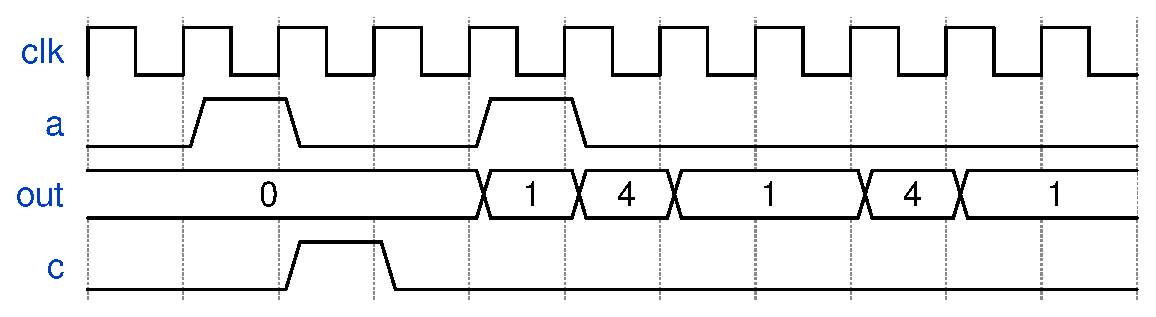
\includegraphics[width=\columnwidth]{figures/example/waveform1.eps}%
	\caption{Waveform Showing the Input-Output Behaviour of the RTL in Fig.~\ref{fig:example}}
\label{intro-waveform}
\end{center}
\end{figure}
%
